\section{Arquitectura de Persistencia de Datos}
\label{sec:base_datos}

La base de datos se modeló y desplegó aplicando principios de integridad referencial rígida y aislamiento de entornos, sentando las bases para escalabilidad en entornos \textit{Cloud}.

\subsection{Modelado Lógico y Orquestación Local}
El modelo de datos lógico fue abstraído utilizando la herramienta DbSchema. Para erradicar discrepancias de dependencias en el equipo de desarrollo, se construyó una infraestructura basada en contenedores gestionada mediante \comando{docker-compose.yml}, garantizando la paridad técnica entre todos los nodos locales de desarrollo. 

\subsection{Estandarización, Tipado y Despliegue en la Nube}
Garantizando el cumplimiento de los estándares de nomenclatura internacionales, el conjunto completo de entidades, tablas y columnas fue redactado estrictamente en inglés. Las entidades mapean de forma precisa objetos principales como \comando{profile}, \comando{profile\_basic}, \comando{countries} y \comando{roles}. 
A nivel de optimización, se erradicó el uso indiscriminado del tipo de dato texto dinámico, implementando \textit{User-Defined Types} (UDTs) y enumeradores (ENUMs). El campo de avatar se adaptó para almacenamiento binario nativo (\comando{bytea}). Finalmente, el esquema y las tablas maestras pre-cargadas (\textit{seeding}) fueron migradas a la infraestructura \textit{Serverless} Neon.tech para soportar la estrategia de CI/CD.

\subsection{Detalle Técnico del Esquema Relacional y Persistencia}
\label{ssec:detalle_db}

En esta subsección se detalla la implementación técnica del modelo de datos, abarcando desde la concepción lógica hasta la creación de estructuras avanzadas en PostgreSQL. Se ha priorizado la integridad semántica de los datos utilizando un enfoque de tipado fuerte soportado nativamente por el motor de base de datos.

A continuación, se presenta la evidencia gráfica del esquema finalizado, así como la definición de dominios, tablas, tipos enumerados y el poblado inicial de catálogos estáticos.

\begin{figure}[htbp]
    \centering
    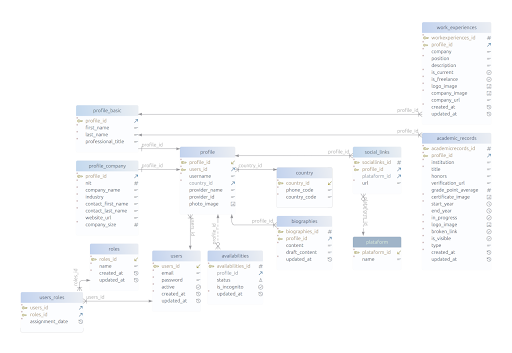
\includegraphics[width=0.7\textwidth]{assets/img/database/db5.png}
    \caption{Modelo Entidad-Relación Lógico Final. Esquema concluido en la herramienta DbSchema, mostrando la topología relacional completa, las llaves primarias (PK) y foráneas (FK) que componen la arquitectura de datos central de la plataforma.}
    \label{fig:db_schema_final}
\end{figure}

\newpage
\begin{figure}[htbp]
    \centering
    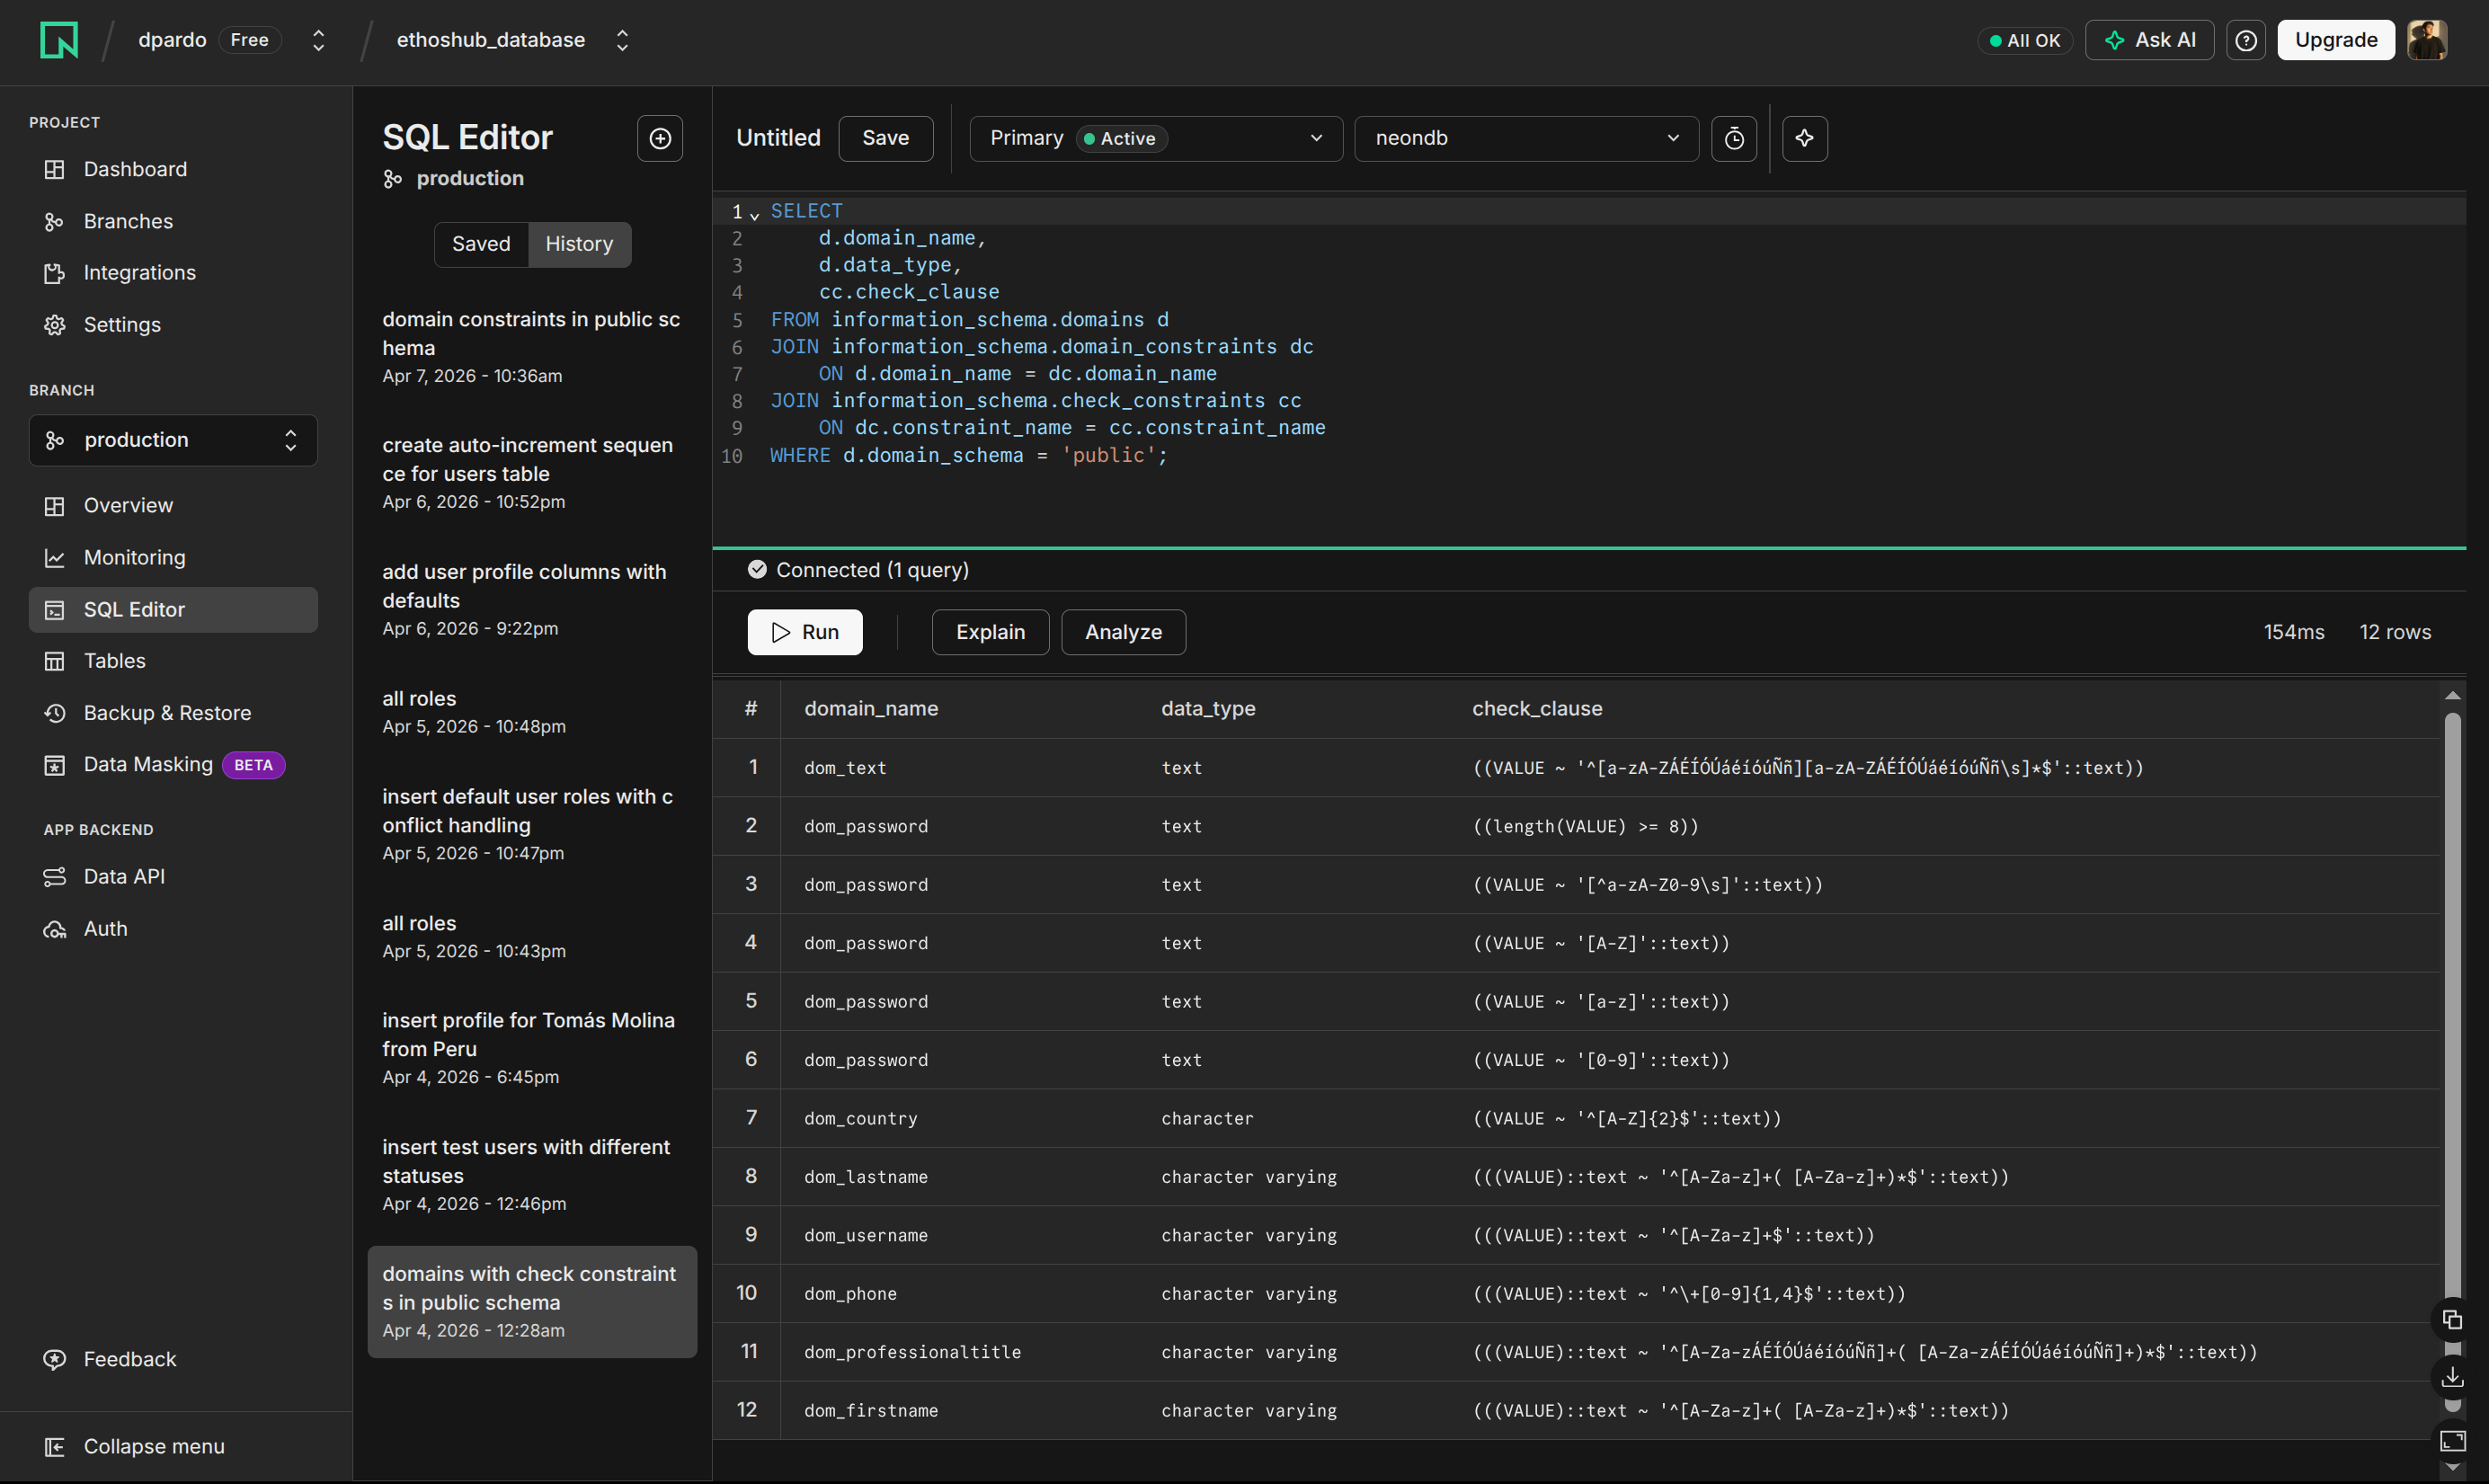
\includegraphics[width=0.7\textwidth]{assets/img/database/db1.png}
    \caption{Creación de Dominios personalizados (\textit{User-Defined Types}). Implementación de restricciones de formato a nivel de base de datos para garantizar la integridad y validación estricta de los campos antes de su persistencia.}
    \label{fig:db_domains}
\end{figure}

\begin{figure}[htbp]
    \centering
    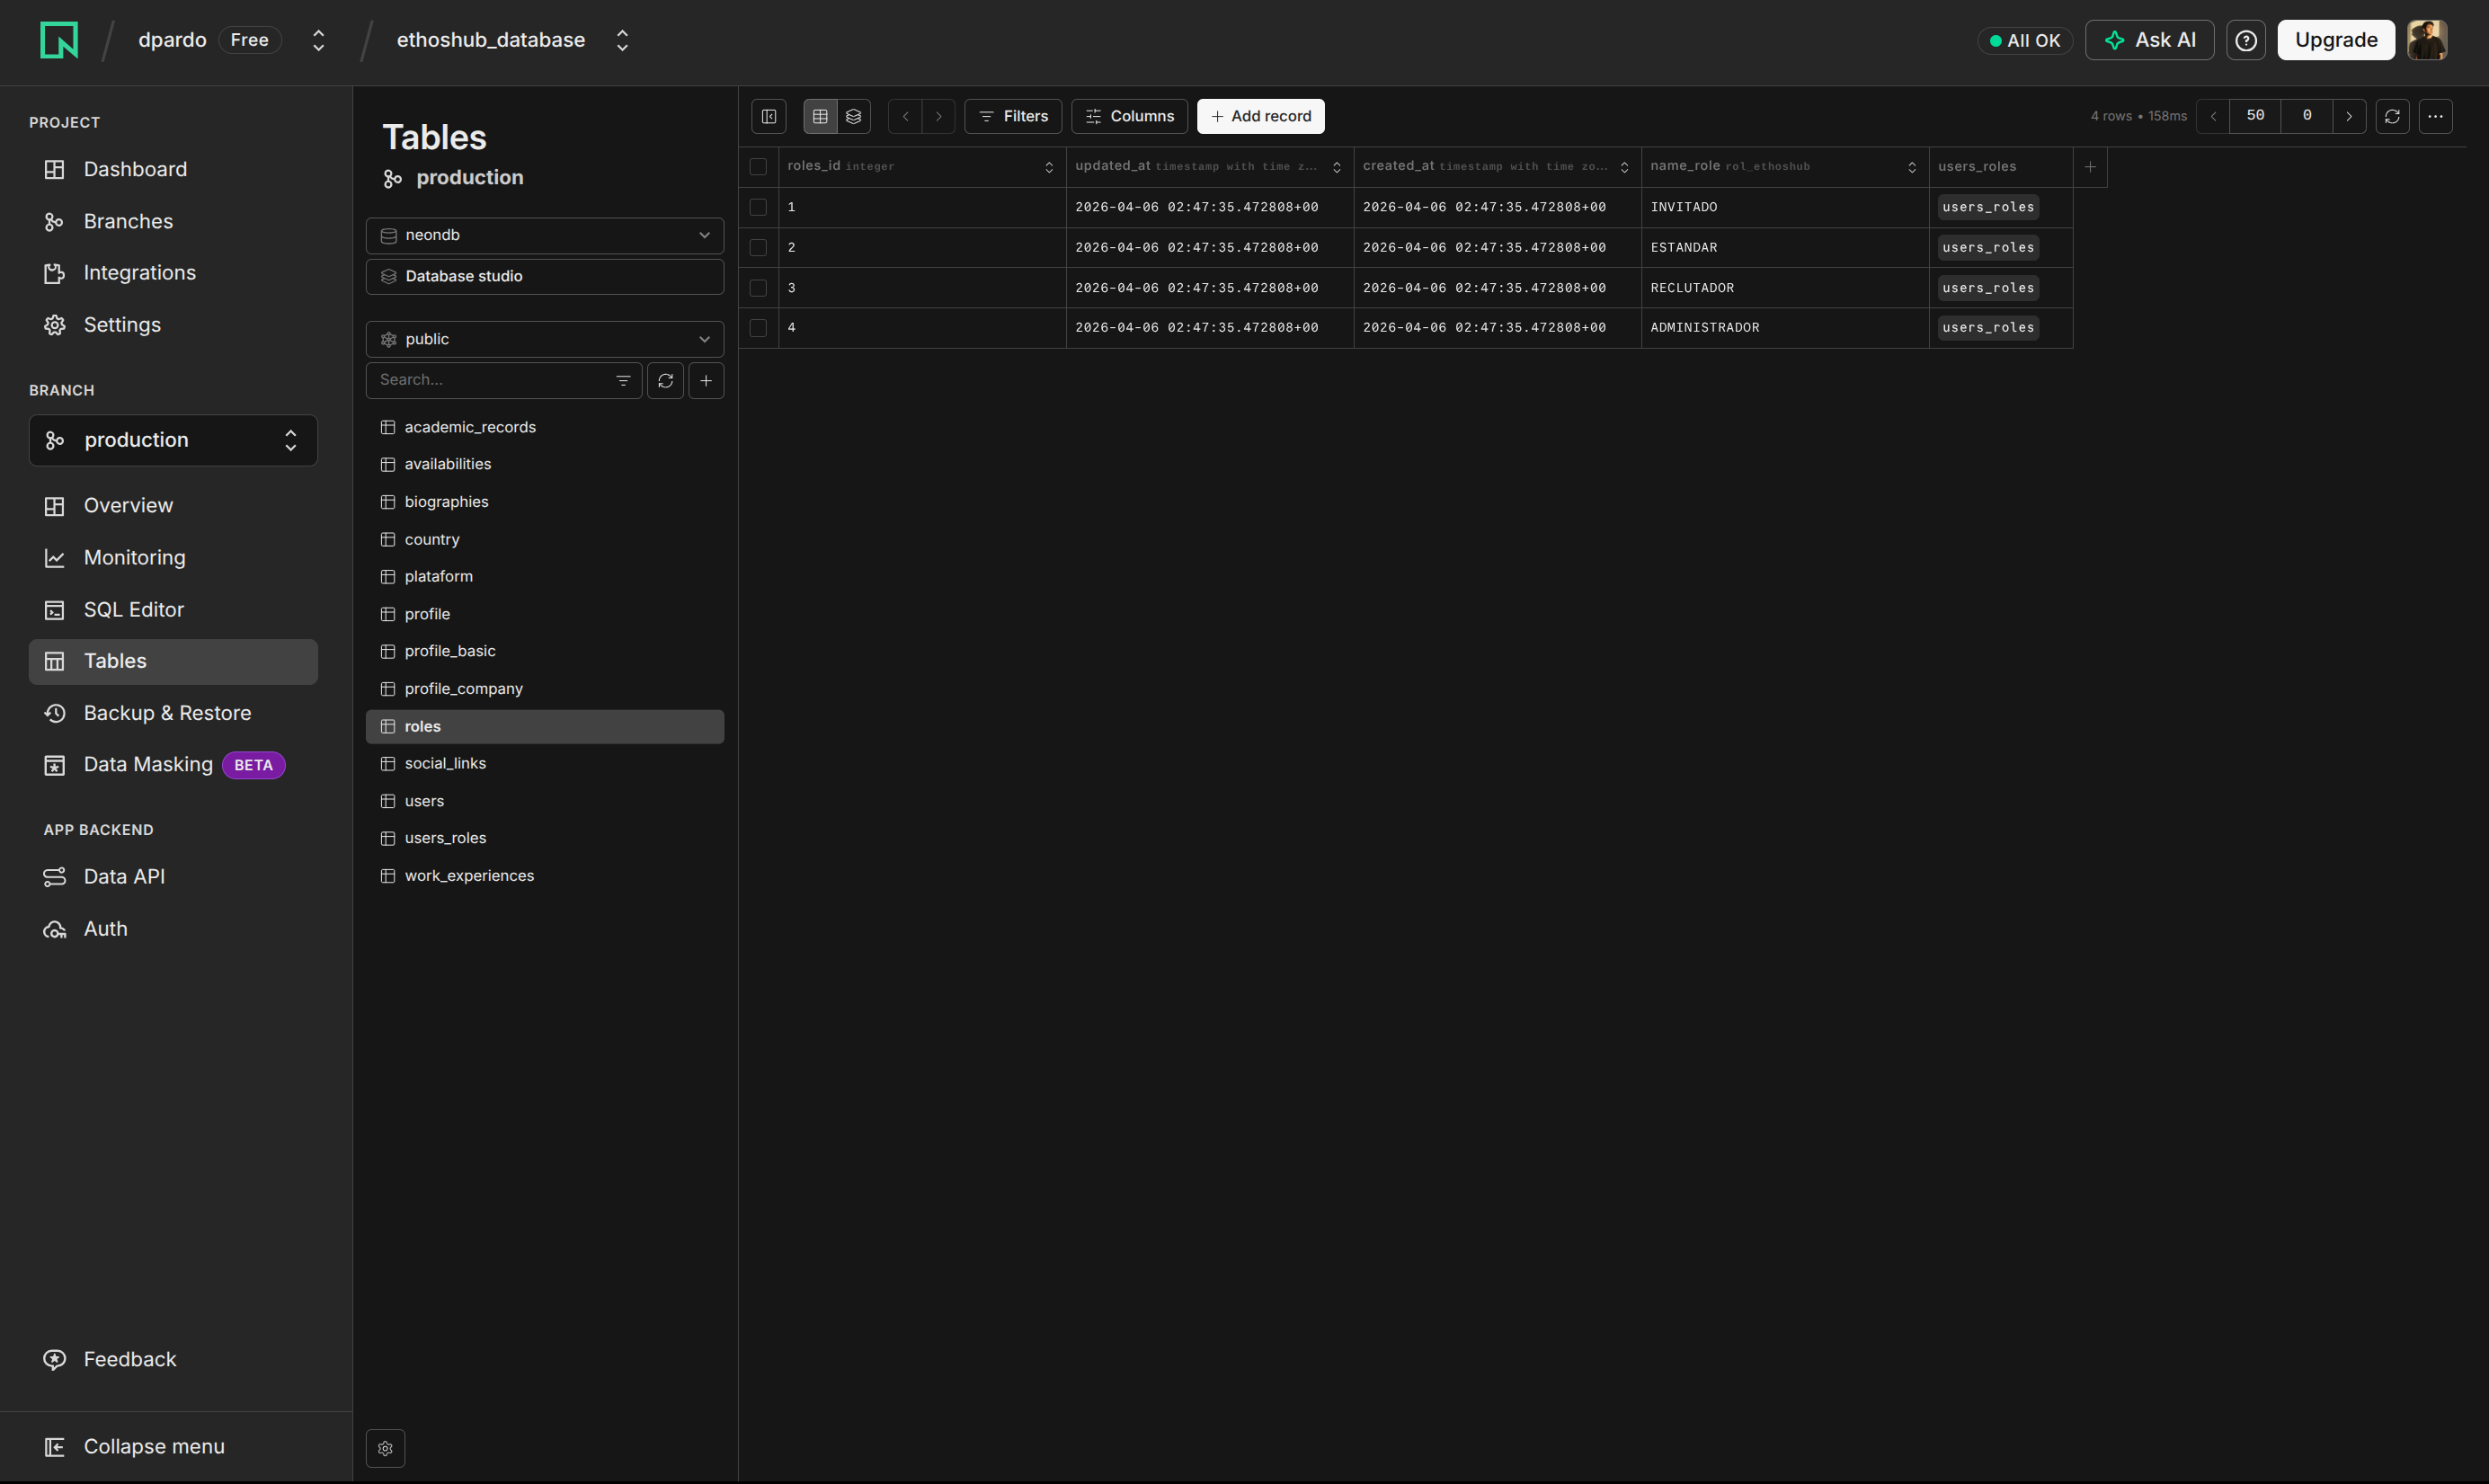
\includegraphics[width=0.7\textwidth]{assets/img/database/db2.png}
    \caption{Estructura de Tablas Físicas. Listado y visualización de las entidades principales ya materializadas en el motor PostgreSQL, diseñadas manteniendo una nomenclatura estandarizada en inglés.}
    \label{fig:db_tables}
\end{figure}

\newpage
\begin{figure}[htbp]
    \centering
    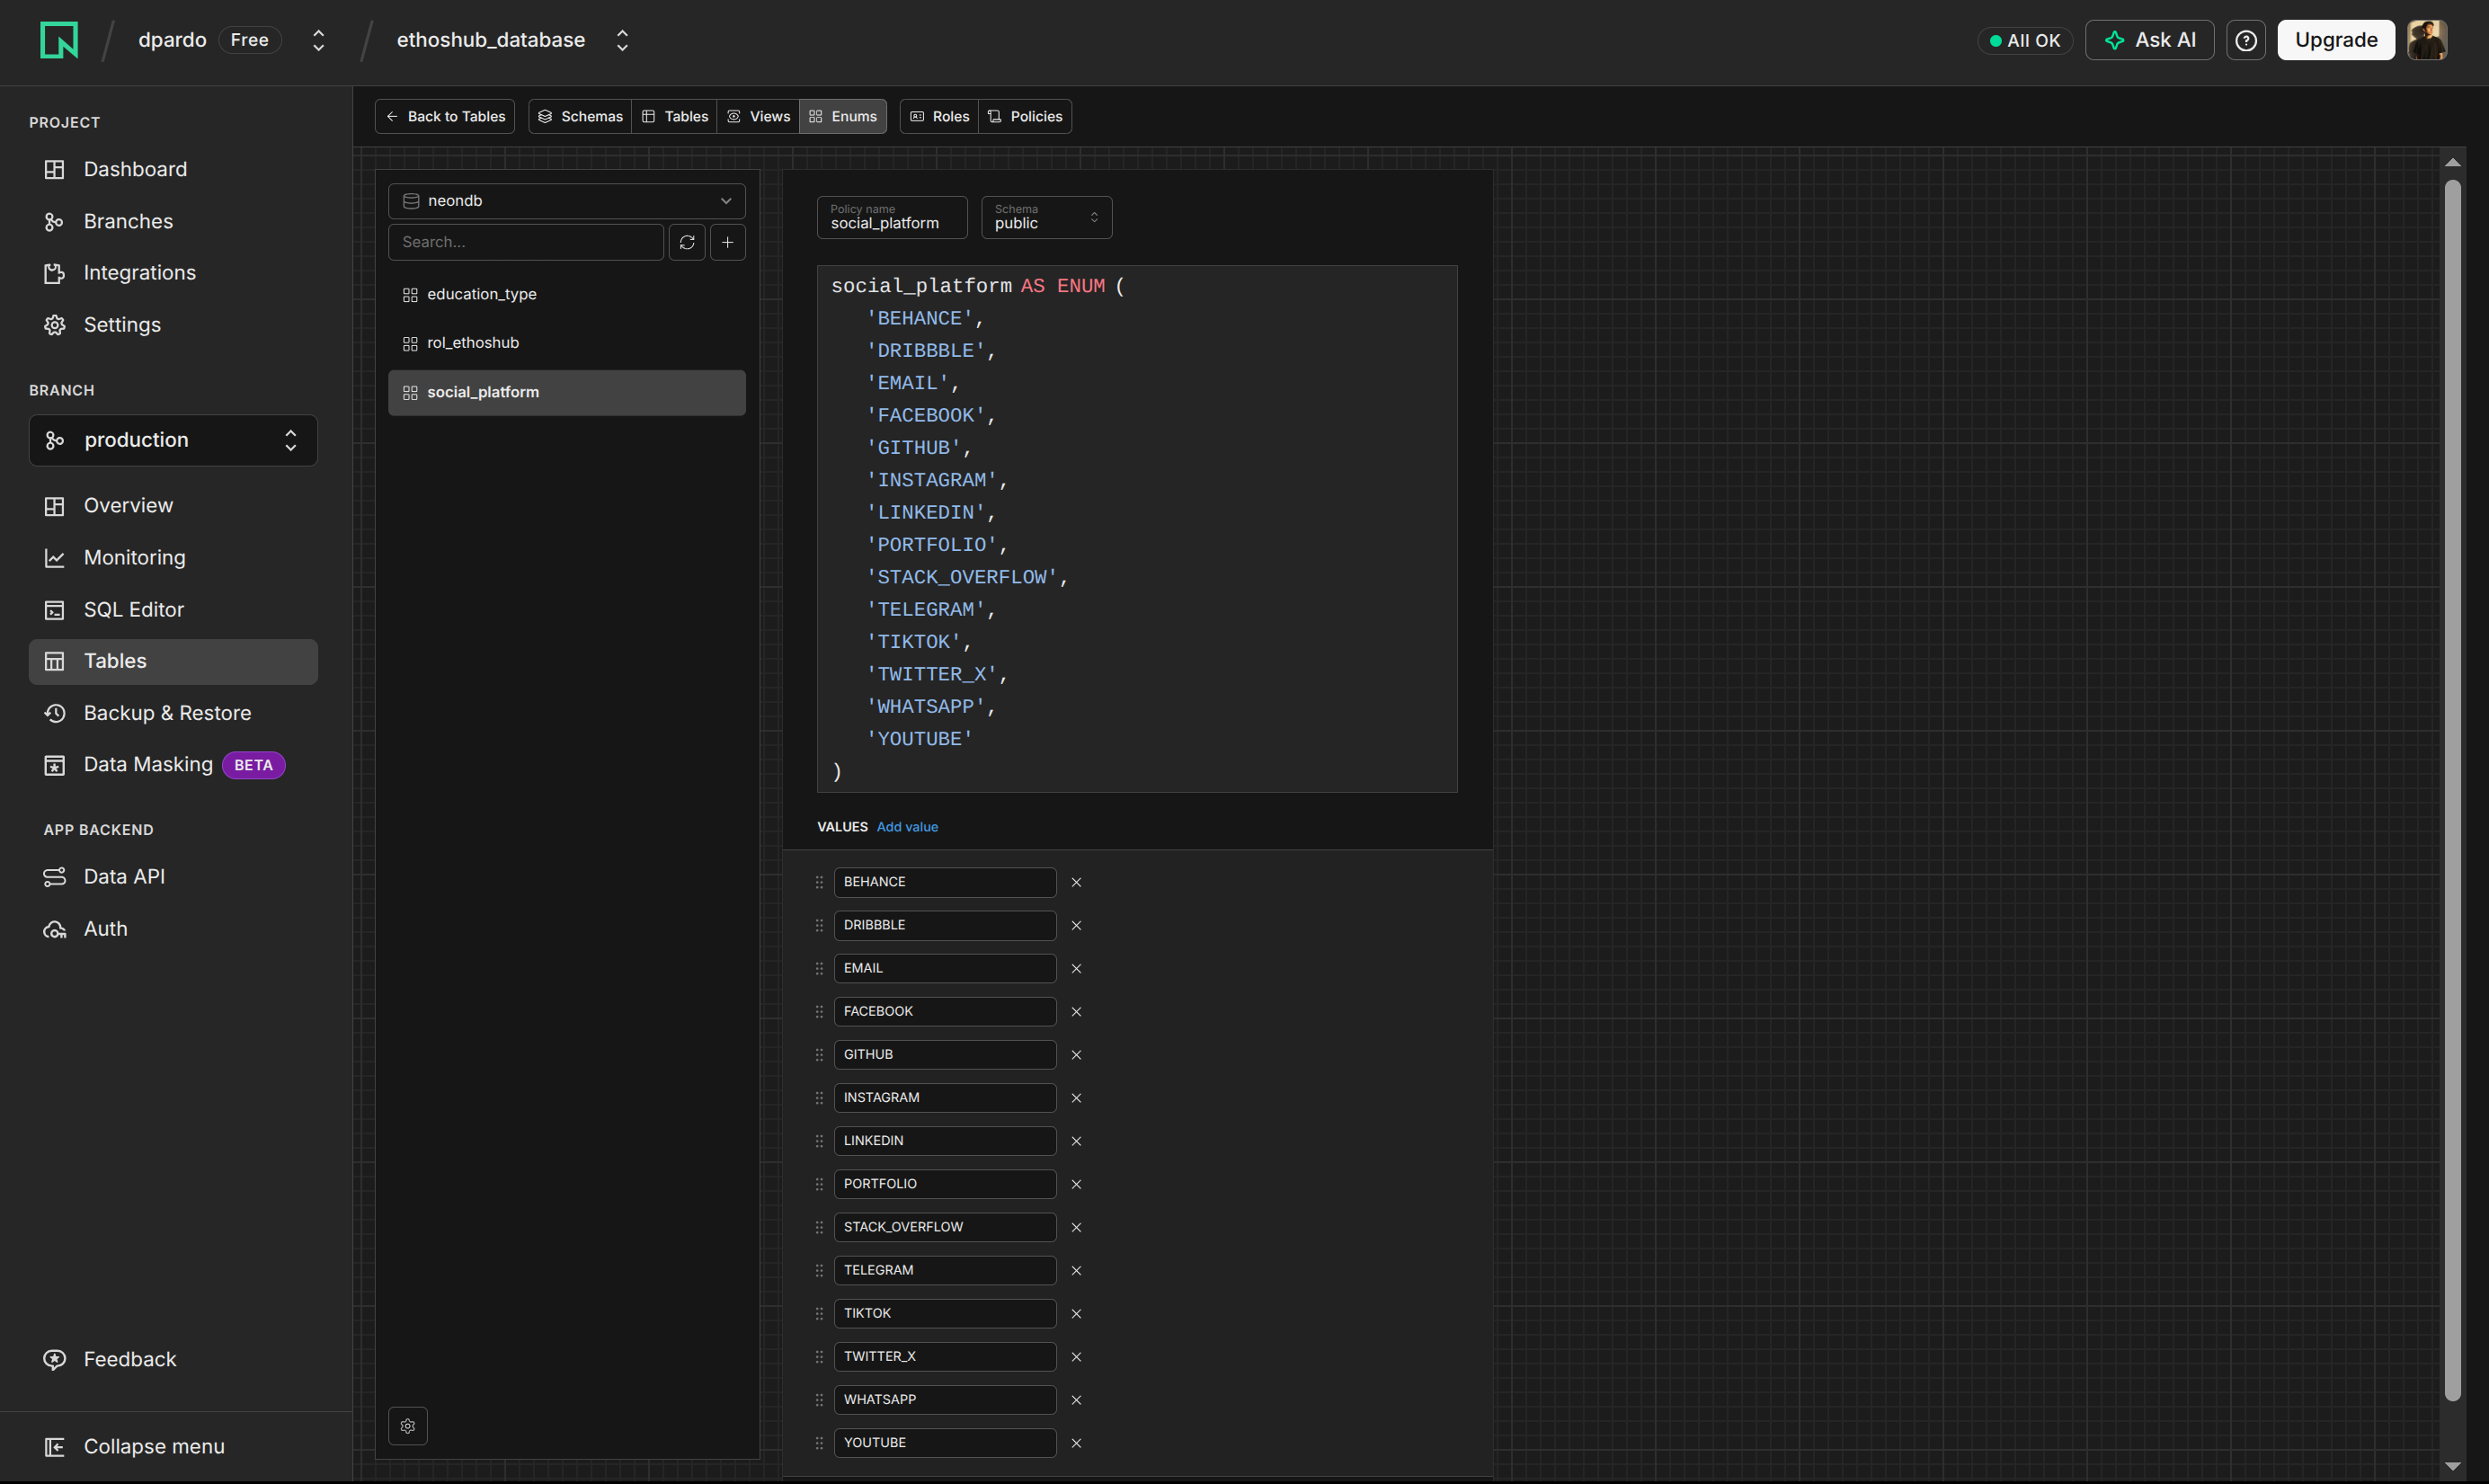
\includegraphics[width=0.7\textwidth]{assets/img/database/db3.png}
    \caption{Definición de Tipos Enumerados (ENUMs). Se evidencia la sustitución de cadenas de texto dinámicas genéricas por conjuntos de datos restrictivos, optimizando el rendimiento de las consultas y previniendo la inserción de estados inválidos.}
    \label{fig:db_enums}
\end{figure}

\begin{figure}[htbp]
    \centering
    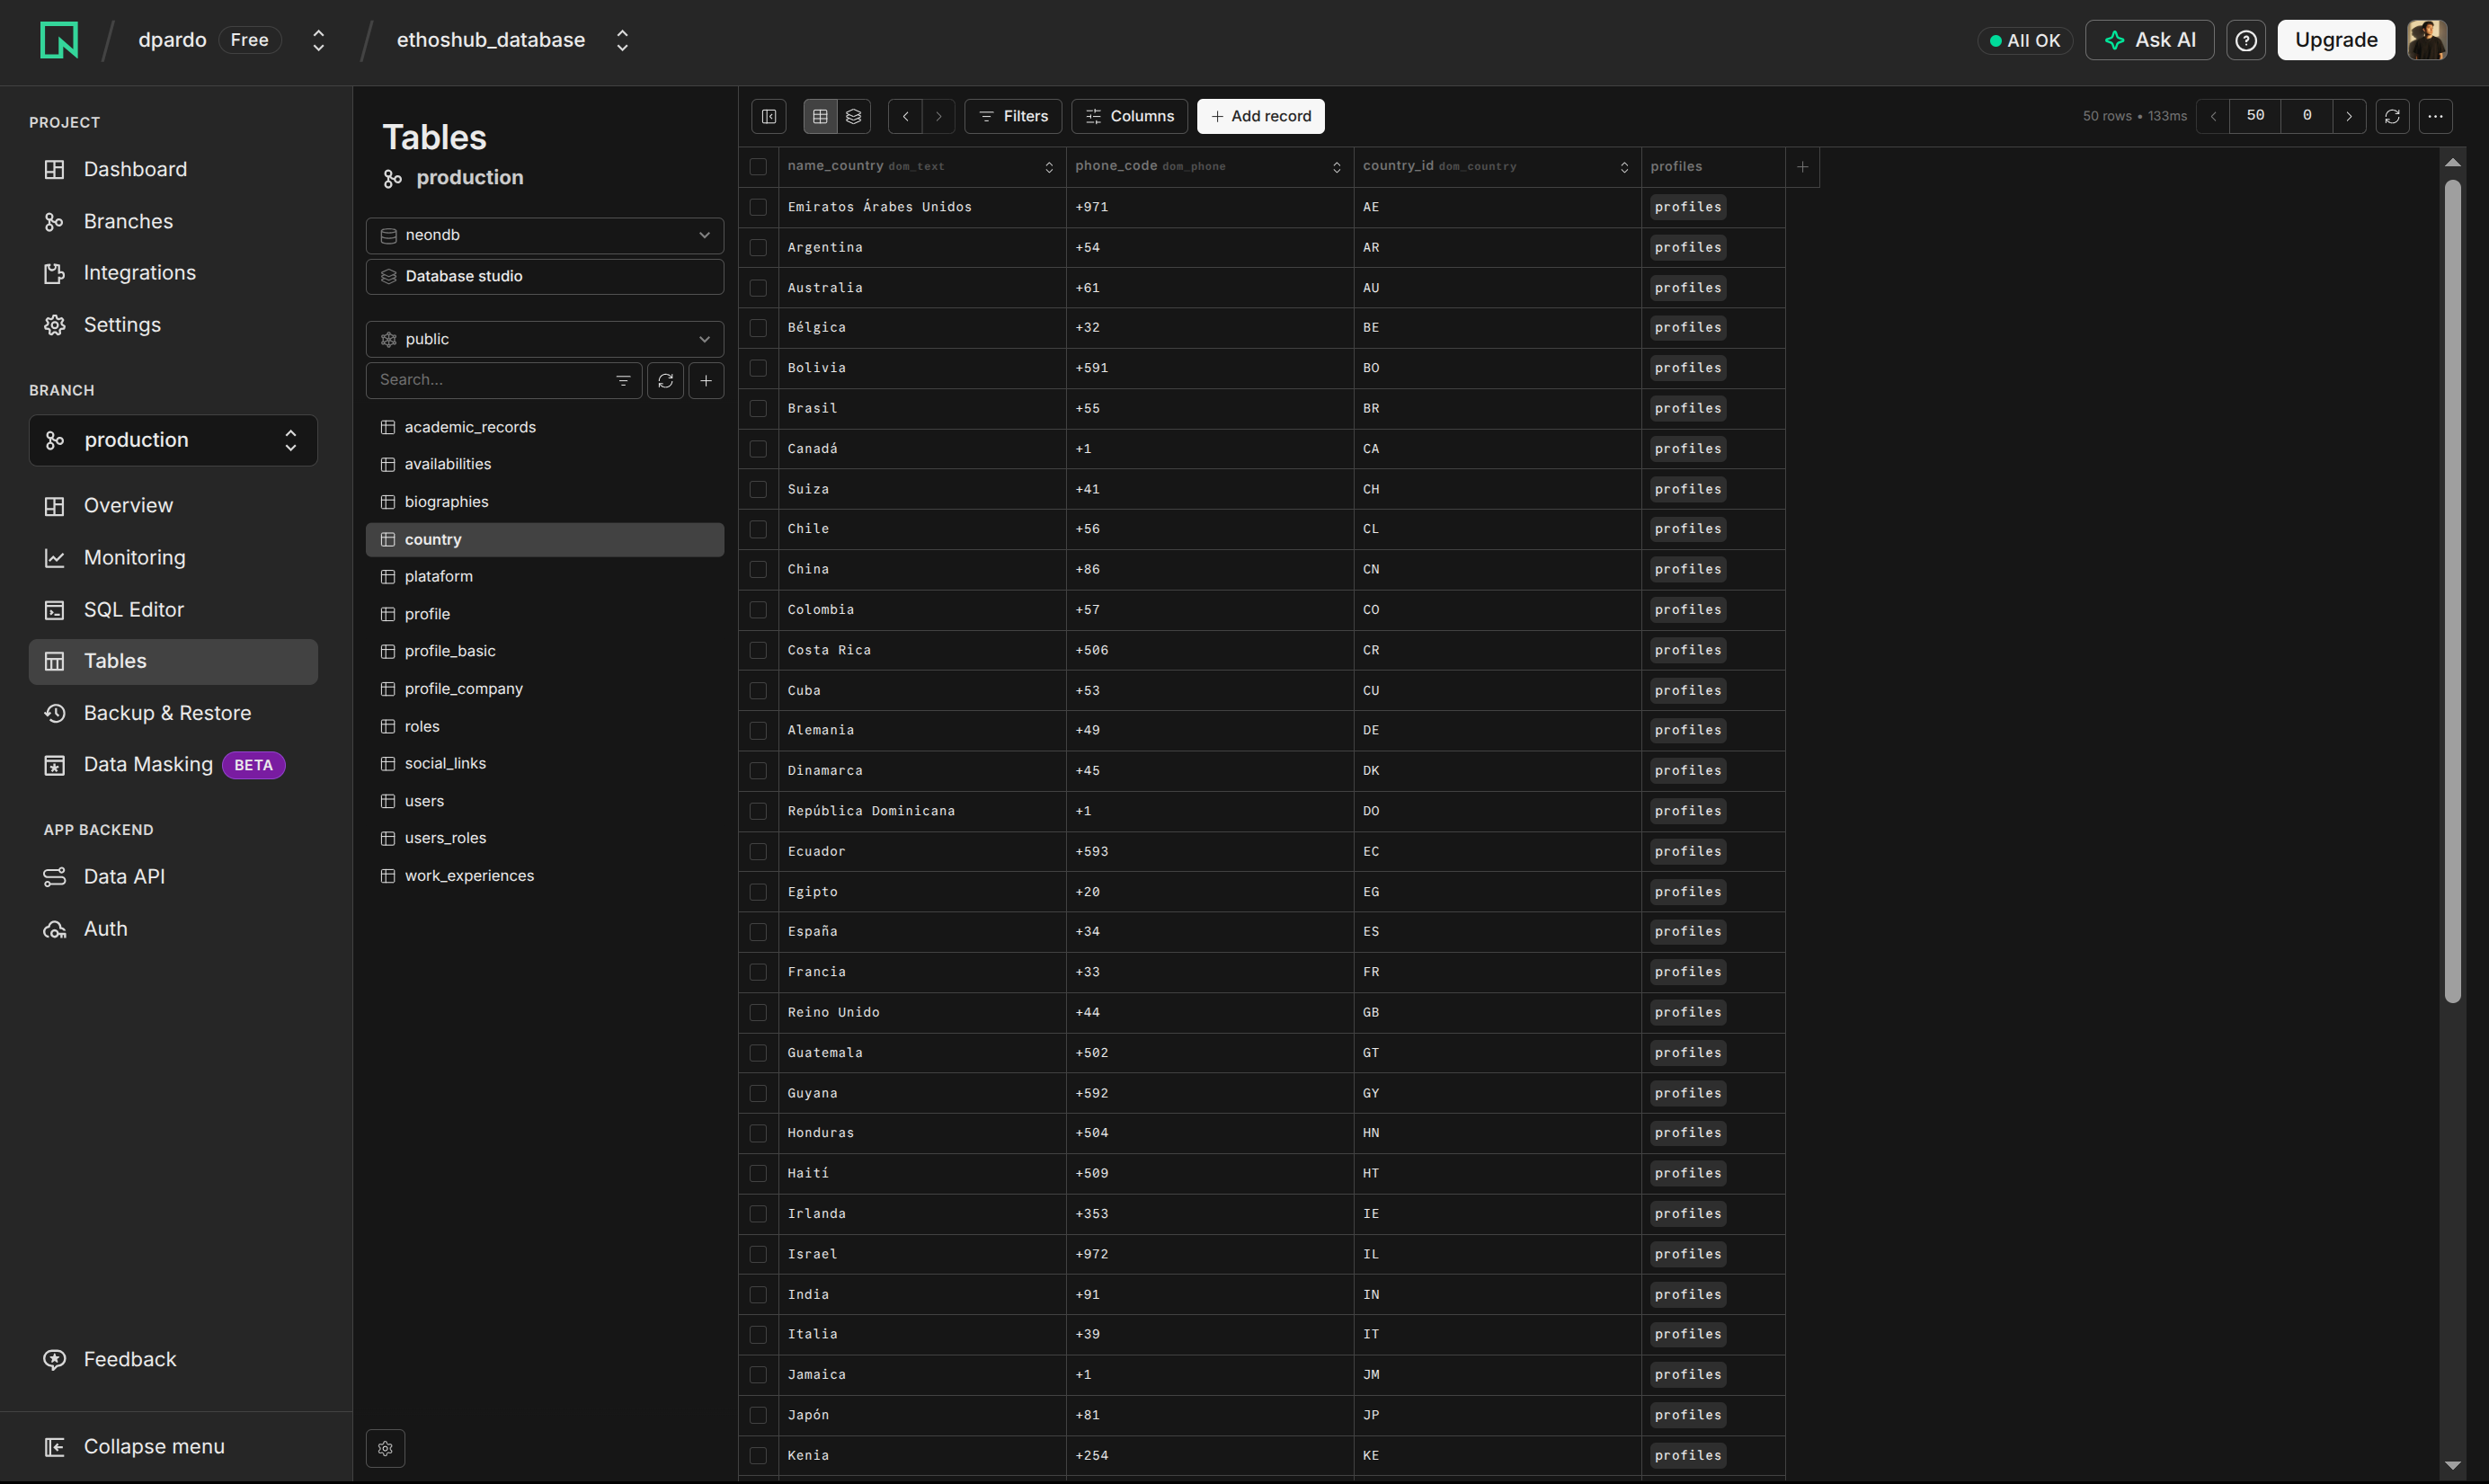
\includegraphics[width=0.7\textwidth]{assets/img/database/db4.png}
    \caption{Poblado Inicial de Datos (\textit{Seeding}). Evidencia de los registros pre-cargados en los diccionarios y catálogos de solo lectura, ejemplificado mediante la inicialización de la tabla \comando{country}.}
    \label{fig:db_seeding_country}
\end{figure}

\begin{NotaTecnica}
La combinación de un modelado lógico riguroso materializado desde DbSchema con la implementación de dominios y ENUMs directamente en el DDL garantiza una capa de persistencia defensiva. Esto reduce significativamente la carga de procesamiento en las validaciones del backend y asegura una escalabilidad óptima y segura para el producto.
\end{NotaTecnica}